\documentclass[11pt]{article}
\usepackage{amsmath,amsfonts,latexsym,graphicx}
\usepackage{fullpage,color}
%\usepackage{text}
%\usepackage{algo}
\usepackage{url,hyperref}
\usepackage{complexity}
\usepackage[linesnumbered,boxed,ruled,vlined]{algorithm2e}

\pagestyle{empty}

\setlength{\oddsidemargin}{0in}
\setlength{\topmargin}{0in}
\setlength{\textwidth}{6.5in}
\setlength{\textheight}{8.5in}

\newtheorem{fact}{Fact}
\newtheorem{lemma}{Lemma}
\newtheorem{theorem}[lemma]{Theorem}
\newtheorem{defn}[lemma]{Definition}
\newtheorem{assumption}[lemma]{Assumption}
\newtheorem{corollary}[lemma]{Corollary}
\newtheorem{prop}[lemma]{Proposition}
\newtheorem{exercise}[lemma]{Exercise}
\newtheorem{claim}[lemma]{Claim}
\newtheorem{remark}[lemma]{Remark}
\newtheorem{prob}{Problem}
\newtheorem{conjecture}{Conjecture}

\newenvironment{note}[1]{\medskip\noindent \textbf{#1:}}%
        {\medskip}

\newenvironment{proof}{\vspace{-0.05in}\noindent{\bf Proof:}}%
        {\hspace*{\fill}$\Box$\par}
\newenvironment{proofsketch}{\noindent{\bf Proof Sketch.}}%
        {\hspace*{\fill}$\Box$\par\vspace{4mm}}
\newenvironment{proofof}[1]{\smallskip\noindent{\bf Proof of #1.}}%
        {\hspace*{\fill}$\Box$\par}

\newcommand{\etal}{{\em et al.}\ }
\newcommand{\assign}{\leftarrow}

\newcommand{\opt}{\textrm{\sc OPT}}
\newcommand{\script}[1]{\mathcal{#1}}
\newcommand{\ceil}[1]{\lceil #1 \rceil}
\newcommand{\floor}[1]{\lfloor #1 \rfloor}


\begin{document}

\setlength{\fboxrule}{.5mm}\setlength{\fboxsep}{1.2mm}
\newlength{\boxlength}\setlength{\boxlength}{\textwidth}
\addtolength{\boxlength}{-4mm}
\begin{center}\framebox{\parbox{\boxlength}{\bf
IIIS 2014 Spring: ATCS - Selected Topics in Optimization \\
Lecture date: ADD DATE, 2009\\
Instructor: Jian Li   \hfill Scribe: YOUR NAME}}\end{center}
\vspace{5mm}

\section{Review}
Recall the following definition about $\epsilon$-net:
A range space $(X;R)$ is a pair consisting of an underlying universe X of objects, and a certain collection
	R of subsets (ranges) of X. 
Furthermore, we focus on those range spaces of finite  VC-dimension; namely, for any finite subset $P\subset X$, the number of distinct sets $r\cap P$,
for $r\in R$, is $O(|P|^d)$, for some constant $d$ (which is upper bounded by the VC-dimension of $(X;R)$).

Then given a range space $(X;R)$, a finite subset $P \subset X$, and a parameter $0 < \epsilon < 1$, an $\epsilon$-net for $P$ (and
$R$) is a subset $N \subseteq P$ with the property that any range $r \in R$ with $|r\cap P|\geq \epsilon|P|$ contains an element
of $N$. 

By last lecture, we have known that for any $(X;R)$, finite subset $P\subset X$ and $\epsilon$, such
	that $(X;R)$ has finite  VC-dimension $d$,
	there is a $\epsilon$-net of size $O(\frac{d}{\epsilon}\log \frac{1}{\epsilon})$. 
This can be done by a random
	sample of $P$ of that size, which could be an $\epsilon$-net with constant probability by
	double sampling tricks. 
Furthermore, the size of $\epsilon$-net for general case is tight.

\section{Construct a $\frac{1}{\epsilon}$-size $\epsilon$-net for halfspaces in $R^3$}


One of the major questions in the theory of $\epsilon$-nets is whether we could have 
	the $\epsilon$-net with a smaller size in normal (geometric) case, instead of considering the general case.
More precisely, the question is whether the factor $\log \frac{1}{\epsilon}$
	 in the upper bound on their size is really necessary.

Here we show, the answer is yes for halfspaces in $R^3$. That is, 
\begin{theorem}\cite{har2014epsilon}
	Given a set $P$ of $n$ points in $R^3$ in general position, and a parameter $0 <  \epsilon<1$, there
	exists an $\epsilon$-net for $(P;H)$ of size $O(\frac{1}{\epsilon})$, where $H$ is the family of all (closed) halfspaces
	(bounded by planes).
\end{theorem} 
It is straightforward to see that the theorem implies the same result for halfplanes in the plane. 
Further, based on projection of hyperboloid, the theorem also can imply that a similar result holds for disks in the plane. 


\subsection{Construction}
Without loss of generality, we only consider an $\epsilon$-net for lower halfspaces.

A symmetric construction will yield an $\epsilon$-net for upper halfspaces, and the union of the two nets will be
an "-net for all halfspaces. Let $H^-$ denote the set of all lower halfspaces.

\newcommand{\F}{\mathcal{F}}
Let $\beta<\frac {1} {22}$ and construct  a maximal collection $\F$ of lower halfspaces with the following properties 
\begin{enumerate}
	\item Each halfspace  $f\in \F$ contains between $\epsilon n$ and $2\epsilon n$ points.
	\item For any pair of distinct halfspaces $h,g\in \F$ , we have $ |h\cap g\cap P |< \beta \epsilon n$.
\end{enumerate}



Then for each halfspace $h \in F$, we construct an $\frac{\beta}{2}$-net $N_h$ for  $(h \cap P;H^-)$, of size
	$O(\frac{1}{\beta}\log \frac{1}{\beta})=O(1)$.
Therefore, we could get the union $N=\bigcup_{h\in\F} N_h$, which is the desired $\epsilon$-net.

\subsection{Proof}
To show $N$ is the desired $\epsilon$-net, 
	it is sufficient for us to prove two things: (1) $N$ is $\epsilon$-net; (2) $|\F|=O(\frac{1}{\epsilon})$. 

First, it is easy to see that $N$ is an $\epsilon$-net.
Without loss of generality, we consider each $h\in R$ containing $\epsilon n$ points (otherwise, shift) and
	all we need to prove is that $h$ must contain a point of $N$.
If $h\in \F$, obviously, $ h$ must contain a point of $N_h$, that is, contain a point of $N$.
If $h\not\in \F$, we know there must exist a $g\in \F$ such that $|h\cap g\cap P|\geq \beta \epsilon n$ (since $\F$ is a maximal subset). 
Then $N_g$ must hit $h\cap g\cap P$, i.e. $N_g$ hits $h$. 
Since $N_g$ is a $\frac{\beta}{2}$-net of $g$ and it hits every group of $\frac{\beta}{2}|g\cap P|= $ nodes in $g\cap P$. 



Second, we prove $|\F|=O(\frac{1}{\epsilon})$. Notice that each hyperplane $h\in \F$ happens in upper envelop. 
Otherwise, suppose to the contrary that there exists 
	$h \in \F$ such that all bounding plane of $h$ lies fully below the envelope. 
Let $v$ be the vertex of the
	envelope closest to $h$. 
Clearly, the union of the three halfspaces $a; b; c \in  \F$ defining $v$ cover $h$; that
is, $h \subset a\cup b\cup c$. 
Hence, we have, at least, one of $|a\cap h|$, $|b\cap h|$, $|c\cap h|$ is larger than $\frac{1}{3} \epsilon n\beta \epsilon n$.


\begin{figure}[htbp]	
		\centering
		\label{g1}
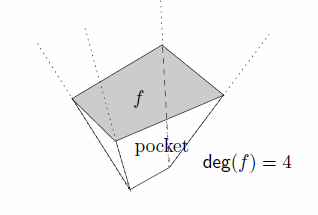
\includegraphics[scale=0.5]{pocket}
\caption{The graph is cited from \cite{har2014epsilon}}
\end{figure}


Now  consider the envelop  as a planar map, which has $|\F|$ faces. 
Define the degree $deg(f)$ as the number of edges of a face $f$. 
Note that, assuming general position, $deg(f)$ is equal to the number of hyperplanes that can be seen from face $f$ (Like Fig. \ref{g1}).
In general, each such plane $g$ seen from $f$ either meets the boundary of $f$ or
	contributes a face to the fully below $f$.
However the latter case is impossible, otherwise, 
	$g$ would not appear on the upper envelope.
 
Let $E$ be the number of edges in the envelop. 
Then by Eular's formula and the fact that $3|\F|\leq 2E$  we have $\sum_{f\in\F} deg(f)\leq 3|\F|-6$. 
Hence, there exist at least $\frac{|\F|}{2}$ faces that have at most $11$ edges, and denote $S^{\leq 11}$ 
	as the set containing such faces. 

For a face in the envelop, define the pocket of $f$ as the set of all halfspaces which contribute to the degree of $f$, i.e. Fig. \ref{g1}. 
Then we have 
\begin{align*}
n&\geq \sum_{f\in \F} (\text{$\sharp$ points contained in the pocket ($f$)})\\
&\geq \sum_{f\in S^{\leq 11}}(\text{$\sharp$ points contained in the pocket ($f$)})\\
&\geq \sum_{f\in S^{\leq 11}}(\epsilon n- 11\beta \epsilon n)\\
&\geq \big|S^{\leq 11}\big|\frac{1}{2}\epsilon n\\
&\geq \frac{1}{4}|\F|\epsilon n
\end{align*}
Thus we have $|\F|\leq \frac{4}{\epsilon}$, which concludes the proof. 



\section{Geometric set cover}

Though the optimal set cover and hitting set
problems are NP-hard, results from $\epsilon$-nets help to give good approximation bounds for these algorithms for
simpler set systems that arise in a geometric context. 

Meggido has proved the geometric set cover problem is \NP-hard in \cite{megiddo1984complexity}. 
Moreover, it has been shown that the problem is NP-Hard to approximate to within a factor of $\Omega(\log n)$.

However, we can take a subset of the problem where S has a bounded dual shattering dimension $\delta^*$.


\subsection{Unweigted version with $O(\log OPT)$ ratio}
The work is done by Clarkson and Varadarajan \cite{clarkson2007improved} by the updating weight trick, 
	which happens often in online learning field. 
	
\begin{algorithm}[h]
	\caption{Hitting set Approx for Unweighted Set Cover}
	\label{alg-set-cover-unweighted}
	Initially, let $w{x} = 1,\forall x\in X$, and let $SOL=\emptyset$\;
	\While{$SOL$ is a set cover}{
		According to the weight, pick a random subset of $R$   of size $O(\frac{\delta^*}{\epsilon} \log \frac{\delta^*}{\epsilon})$\;
		\If{$\exists p\in X$ is uncovered}
		{
			\If{$w(R_p)\leq \epsilon w(R)$}
				{
					$w(R_p)=2w(R_p)$\;
				}
		}
	}%while
	{\bf Return} $\bigoplus$\;

\end{algorithm}
\cite{har2012weighted}




BTW, there is a related note \cite{GeometricSetCover} which writes the same proof in a different way form this note. 
Readers may find more inspiring things from it.  


\section{Solve LP with fixed number of variables -- Seidel Algorithm}




\begin{algorithm}[h]
\caption{An Algorithm}
\label{algo2}
Initially, let $\mathcal{L} = 0$\;
\While{$a>b$}{
    \For{$m = 1,2,\ldots, s+1$}{
        $\Theta=\Xi$\;
    }
   $\clubsuit\diamondsuit\heartsuit\spadesuit$\;
    \If{$b<a$}{ 
        Do nothing\;
    }
}%while
{\bf Return} $\bigoplus$\;
\cite{har2012weighted}
\end{algorithm}
\cite{Seidel}
\bibliographystyle{plain}
\bibliography{a}
%% To add references, uncomment the following two lines and
%% add the relevant bibitems.

\end{document} 